\documentclass{article}
\usepackage[utf8]{inputenc}
\usepackage{graphicx}

% change reference style to [1], remove stupid sorting, language changed so date in ddmmyyyy
\usepackage[backend=biber, style=numeric, sorting=none, language=australian]{biblatex}
\addbibresource{References.bib}

\title{Detecting User Engagement Using \\ Mouse Tracking Data:\\
    \large Project Specification
}
\author{David Saunders (910995)}
\date{April 2020}

\begin{document}
\maketitle

\begin{abstract} 
    Write abstract here
\end{abstract}

\tableofcontents

\section*{Mark scheme}
This coursework contributes 50\% of the mark for the module. The size is
approximately 5000 words (excluding references) – due on Wednesday 29
April 2020 (11:00 am).

This report should give a literature review over your project and describe
any background research that you have carried out. You should state the motivation and aims of the project. It should include a complete specification
of your project. It should describe the project clearly and the components
of the work which need to be developed. An outline project plan for the
summer should be included. This plan should take into account the development methodology being used. You should provide a risk analysis for the
project. You should view this document as providing the plan for the work
you expect to carry out over the summer.

\section{Literature review}

Write section 1 here \cite{torsney2011tuner} and talk about figure \ref{fig:test}.

This can pretty much be the review I did for the first assignment. 

\begin{figure}[ht]
    \centering
    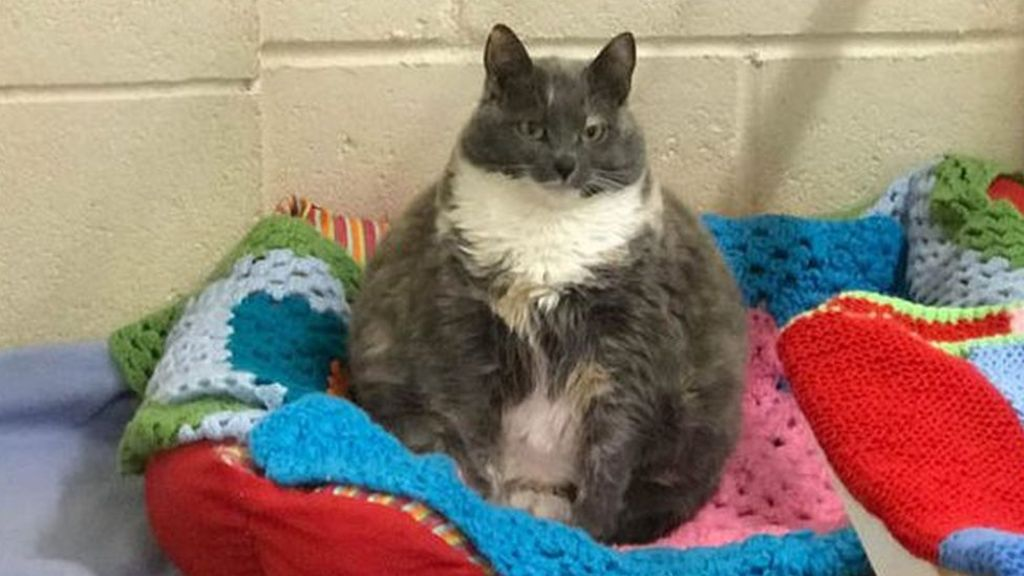
\includegraphics[scale=0.35]{Test.JPG}
    \caption{This will be a figure showcasing some of my work}
    \label{fig:test}
\end{figure}

\section{Background Research}
Anything I've looked at with help for mouse data classification algorithms? 


\section{Motivation and Aims of project}
Can copy from presentation slides but fill in so they're more wordy.

\subsection{Motivation}

People are lazy. 
Often don't pay much attention 
Is there any way of measuring people's attention?

Why mouse data?
Mouse cursor position is strongly correlated with eye position. 
One paper calls it a “poor man's eye-tracker” [find]
Bulky expensive equipment for eye tracking is expensive and very obtrusive.
Hawthorn / observer effect - People react differently when being observed. 
Less obtrusive mouse tracking can make people feel less tracked and act more naturally. 
Could even not tell them (legal ethical repercussions)!

\subsection{Aims of project}

The aims of what I want to achieve in the project will be as follows:
\begin{itemize}
    \item Visualise, analyse and understand the data results.
    \item Use the data to train machine learning models to classify users between 2 groups.
    \item Combine the data and methods from the study data with other datasets to create a more robust model.
    \item Stretch goal? Test methods and models developed with other applications?
\end{itemize}

Talk here about how I will achieve each aim, then describe the components of the project that I will need to complete.
Try and link each component of the project to an aim.

Machine learning methods
    SVM
    Natural Language Processing
    N-Grams
    LSTM Neural Networks
    Markov models
Deal with Imbalances in classes
    Sampling
    Oversampling, Undersampling
Other mouse data sources

Applications
A good system developed could be used for other tasks to monitor attention - E.g. Survey Monika made us do. Not just for joes ice-cream
Have to decide on the trade off between a good narrow (is this the right word) classifier between attention or not and a more generalised model that can work on any task.
What I mean by that is I can model the html elements / sliders to see how users interacted to see the stock prices, or I can generalise to any such task involving mouse data.


\section{Project plan}

\subsection{Development methodology}
Discuss software life cycle methodologies with Jacques.
An agile methodology such as scrum would probably be best but am I constrained  by this specification document?

\begin{figure}[ht]
    \centering
    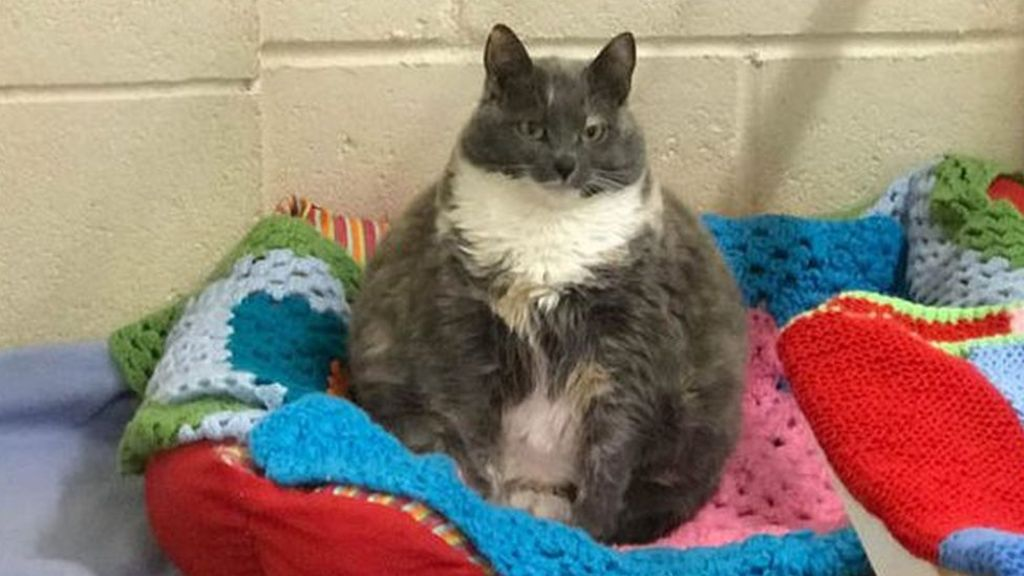
\includegraphics[scale=0.35]{Test.JPG}
    \caption{A Gantt chart showing the planned milestones of the project.}
    \label{fig:Gantt}
\end{figure}

\section{Risk Analysis}
Copy this from my project last year.

\begin{table}[ht]
    \caption{A risk analysis table}
    \centering
    \begin{tabular}{lllll}
     Risk   Likelihood  Impact  &  \\
     &      Low         High       &  \\
     &      &           &       &  \\
     
    \end{tabular}
\end{table}


Risks: 
- BIGGEST we find that there is no correlation between attendtion and mouse data and nothing is prooved.
- COID19 effecting the UK more. - I was considering running more lab studies to get more data but the shutdown has stopped that ambishion.
    It has already effected, anything worse like close family and elderly parents getting ill so supervisor or me would be a risk.
    Plan ahead, wash hands.


\section{Conclusion}

Measuring user engagement is challenging
Mouse data can help us solve that issue by showing user attention
Data Science techniques could be used to help classify the data (Not SVM)


\printbibliography

\end{document}